\begin{frame}{Simulation}
  \small{We run simulations of $3$ repeating patterns: square, hexagon, octagon-square.
    \begin{enumerate}
    \item For each lattice pattern, the number of robots $n=50,100,150,200,250$.
    \item For each $n$, we run $50$ trials with random initial poses.
    \end{enumerate}
  }
  \only<1>{
    \begin{figure}
      \centering
      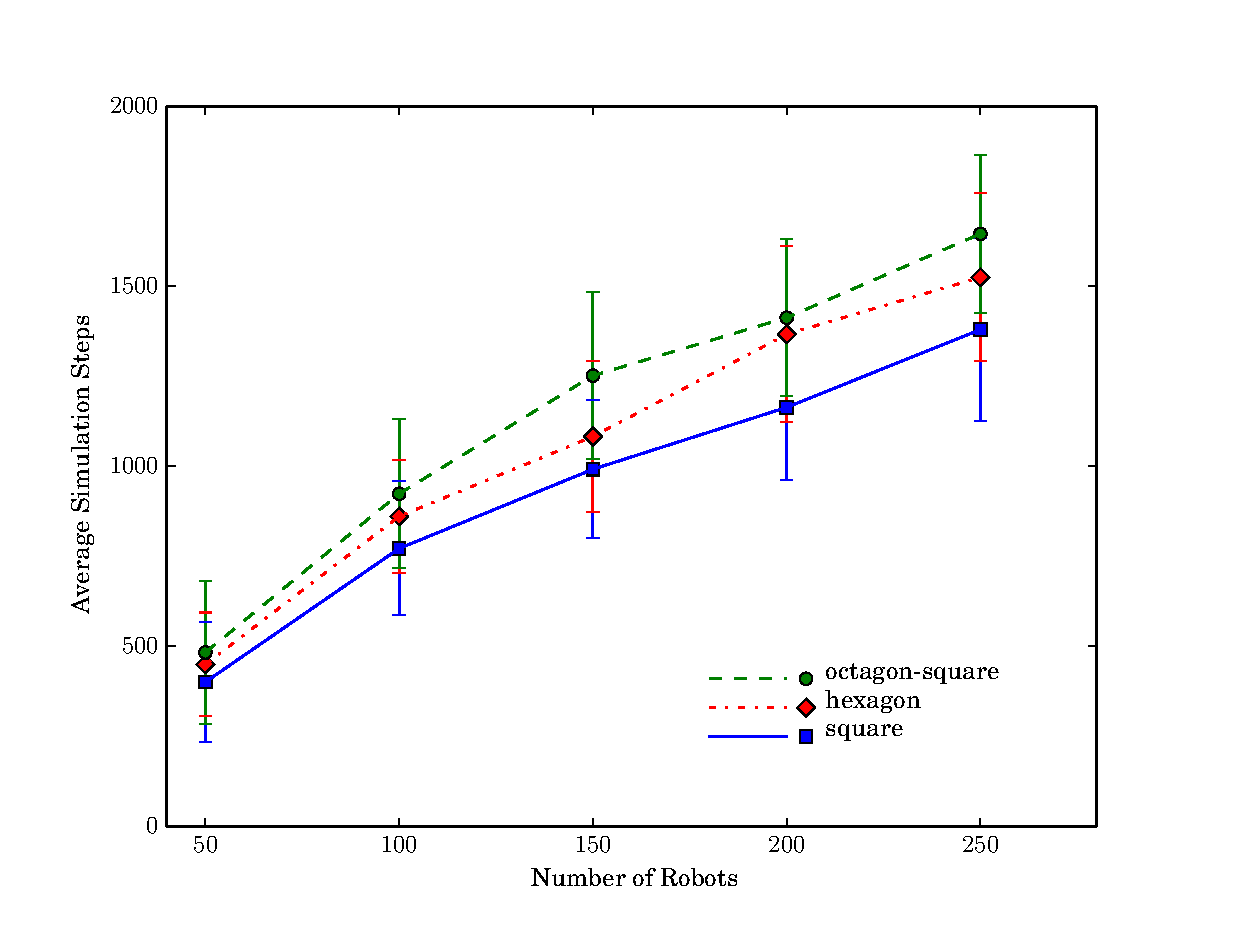
\includegraphics[width=0.65\textwidth]{figs/exp_time}
      %\caption{Average execution time and its standard deviation of forming repeated lattice patterns of square, hexagon and octagon-square.} 
    \end{figure}
  }
  \only<2>{
    \begin{figure}
      \centering
      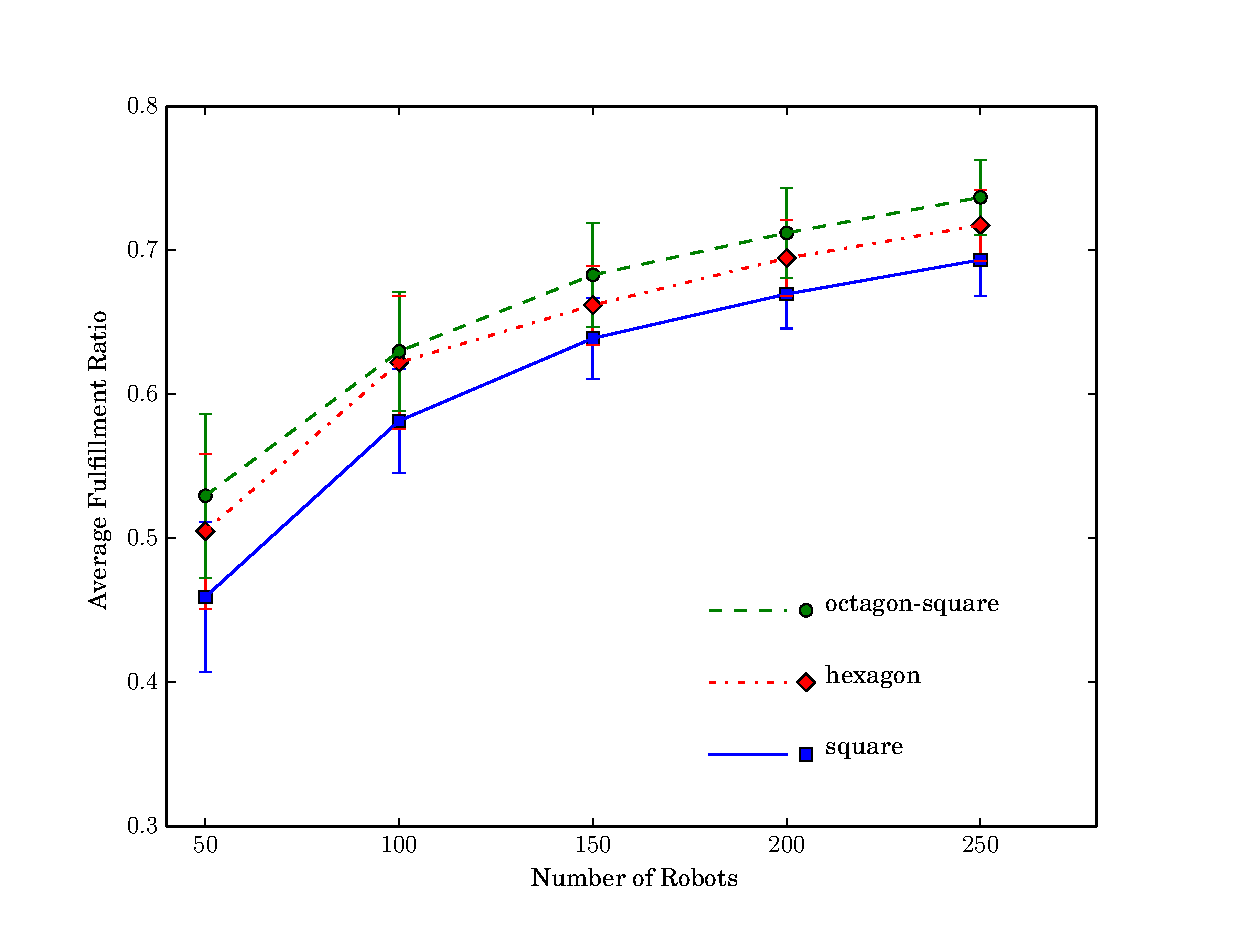
\includegraphics[width=0.65\textwidth]{figs/exp_qual}
      %\caption{Average fulfillment ratio and its standard deviation of forming lattice patterns of square, hexagon and octagon-square.} 
    \end{figure}
  }
\end{frame}